% \captionsetup[figure]{list=no}   % don't add appendix figs to LoF
% \captionsetup[table]{list=no}    % don't add appendix tables to LoT
\addtocontents{toc}{\protect\setcounter{tocdepth}{0}}
\chapter{Additional Results}
\label{chap:appendix}

This appendix provides supplementary results for all experiments described in Chapter~\ref{chap:experiments}. For the Sentinel-2 model training, confusion matrices for the remaining normalization strategies are provided. For the binary VEN$\mu$S experiments, confusion matrices are omitted as they are fully determined by the recall values already reported in the metrics tables, and their visual representation adds limited value, as these strategies do not represent the best performing result. For all experiments, additional visual prediction examples are provided for the best performing normalization strategy only.

\section{Sentinel-2 Model Training}
\label{app:s2}


\begin{figure}[H]
    \centering
    \begin{subfigure}{0.48\textwidth}
        \centering
        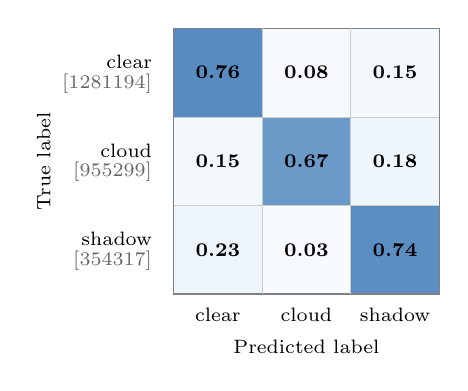
\begin{tikzpicture}[scale=0.75]
        \definecolor{cellhigh}{RGB}{33,102,172}
\definecolor{celllow}{RGB}{214,232,246}
\definecolor{cellzero}{RGB}{247,251,255}
\fill[cellhigh!75] (0.0,3.0) rectangle (1.5,4.5);
\node[black, font=\scriptsize\bfseries] at (0.75,3.75) {0.76};
\fill[celllow!20] (1.5,3.0) rectangle (3.0,4.5);
\node[black, font=\scriptsize\bfseries] at (2.25,3.75) {0.08};
\fill[celllow!30] (3.0,3.0) rectangle (4.5,4.5);
\node[black, font=\scriptsize\bfseries] at (3.75,3.75) {0.15};
\fill[celllow!29] (0.0,1.5) rectangle (1.5,3.0);
\node[black, font=\scriptsize\bfseries] at (0.75,2.25) {0.15};
\fill[cellhigh!66] (1.5,1.5) rectangle (3.0,3.0);
\node[black, font=\scriptsize\bfseries] at (2.25,2.25) {0.67};
\fill[celllow!36] (3.0,1.5) rectangle (4.5,3.0);
\node[black, font=\scriptsize\bfseries] at (3.75,2.25) {0.18};
\fill[celllow!45] (0.0,0.0) rectangle (1.5,1.5);
\node[black, font=\scriptsize\bfseries] at (0.75,0.75) {0.23};
\fill[cellzero] (1.5,0.0) rectangle (3.0,1.5);
\node[black, font=\scriptsize\bfseries] at (2.25,0.75) {0.03};
\fill[cellhigh!74] (3.0,0.0) rectangle (4.5,1.5);
\node[black, font=\scriptsize\bfseries] at (3.75,0.75) {0.74};
\draw[black!50, line width=0.5pt] (0,0) rectangle (4.5,4.5);
\draw[black!20, line width=0.3pt] (1.5,0) -- (1.5,4.5);
\draw[black!20, line width=0.3pt] (0,1.5) -- (4.5,1.5);
\draw[black!20, line width=0.3pt] (3.0,0) -- (3.0,4.5);
\draw[black!20, line width=0.3pt] (0,3.0) -- (4.5,3.0);
\node[font=\scriptsize] at (0.75,-0.35) {clear};
\node[font=\scriptsize] at (2.25,-0.35) {cloud};
\node[font=\scriptsize] at (3.75,-0.35) {shadow};
\node[anchor=east, font=\scriptsize] at (-0.2,3.93) {clear};
\node[anchor=east, font=\scriptsize, black!60] at (-0.2,3.57) {[1281194]};
\node[anchor=east, font=\scriptsize] at (-0.2,2.43) {cloud};
\node[anchor=east, font=\scriptsize, black!60] at (-0.2,2.07) {[955299]};
\node[anchor=east, font=\scriptsize] at (-0.2,0.9299999999999999) {shadow};
\node[anchor=east, font=\scriptsize, black!60] at (-0.2,0.5700000000000001) {[354317]};
\node[font=\scriptsize] at (2.25,-0.9) {Predicted label};
\node[rotate=90, font=\scriptsize] at (-2.2,2.25) {True label};
        \end{tikzpicture}
        \caption{Without normalization.}
        \label{fig:s2_confusion_raw}
    \end{subfigure}
    \hfill
    \begin{subfigure}{0.48\textwidth}
        \centering
        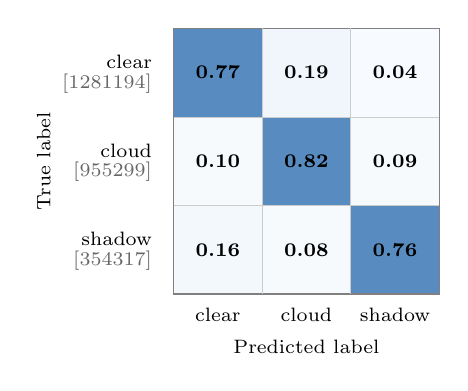
\begin{tikzpicture}[scale=0.75]
        \definecolor{cellhigh}{RGB}{33,102,172}
\definecolor{celllow}{RGB}{214,232,246}
\definecolor{cellzero}{RGB}{247,251,255}
\fill[cellhigh!75] (0.0,3.0) rectangle (1.5,4.5);
\node[black, font=\scriptsize\bfseries] at (0.75,3.75) {0.77};
\fill[celllow!37] (1.5,3.0) rectangle (3.0,4.5);
\node[black, font=\scriptsize\bfseries] at (2.25,3.75) {0.19};
\fill[cellzero] (3.0,3.0) rectangle (4.5,4.5);
\node[black, font=\scriptsize\bfseries] at (3.75,3.75) {0.04};
\fill[celllow!20] (0.0,1.5) rectangle (1.5,3.0);
\node[black, font=\scriptsize\bfseries] at (0.75,2.25) {0.10};
\fill[cellhigh!75] (1.5,1.5) rectangle (3.0,3.0);
\node[black, font=\scriptsize\bfseries] at (2.25,2.25) {0.82};
\fill[celllow!20] (3.0,1.5) rectangle (4.5,3.0);
\node[black, font=\scriptsize\bfseries] at (3.75,2.25) {0.09};
\fill[celllow!32] (0.0,0.0) rectangle (1.5,1.5);
\node[black, font=\scriptsize\bfseries] at (0.75,0.75) {0.16};
\fill[celllow!20] (1.5,0.0) rectangle (3.0,1.5);
\node[black, font=\scriptsize\bfseries] at (2.25,0.75) {0.08};
\fill[cellhigh!75] (3.0,0.0) rectangle (4.5,1.5);
\node[black, font=\scriptsize\bfseries] at (3.75,0.75) {0.76};
\draw[black!50, line width=0.5pt] (0,0) rectangle (4.5,4.5);
\draw[black!20, line width=0.3pt] (1.5,0) -- (1.5,4.5);
\draw[black!20, line width=0.3pt] (0,1.5) -- (4.5,1.5);
\draw[black!20, line width=0.3pt] (3.0,0) -- (3.0,4.5);
\draw[black!20, line width=0.3pt] (0,3.0) -- (4.5,3.0);
\node[font=\scriptsize] at (0.75,-0.35) {clear};
\node[font=\scriptsize] at (2.25,-0.35) {cloud};
\node[font=\scriptsize] at (3.75,-0.35) {shadow};
\node[anchor=east, font=\scriptsize] at (-0.2,3.93) {clear};
\node[anchor=east, font=\scriptsize, black!60] at (-0.2,3.57) {[1281194]};
\node[anchor=east, font=\scriptsize] at (-0.2,2.43) {cloud};
\node[anchor=east, font=\scriptsize, black!60] at (-0.2,2.07) {[955299]};
\node[anchor=east, font=\scriptsize] at (-0.2,0.9299999999999999) {shadow};
\node[anchor=east, font=\scriptsize, black!60] at (-0.2,0.5700000000000001) {[354317]};
\node[font=\scriptsize] at (2.25,-0.9) {Predicted label};
\node[rotate=90, font=\scriptsize] at (-2.2,2.25) {True label};
        \end{tikzpicture}
        \caption{Fixed Z-score with Sentinel-2 statistics.}
        \label{fig:s2_confusion_s2}
    \end{subfigure}
    \caption[Confusion matrices for S2 models on the S2 test set.]{Confusion matrices for the S2 models on the S2 test set. Values are normalized by row.}
    \label{fig:s2_confusion_app}
\end{figure}



\begin{figure}[H]
    \centering
        \begin{subfigure}{\textwidth}
        \centering
        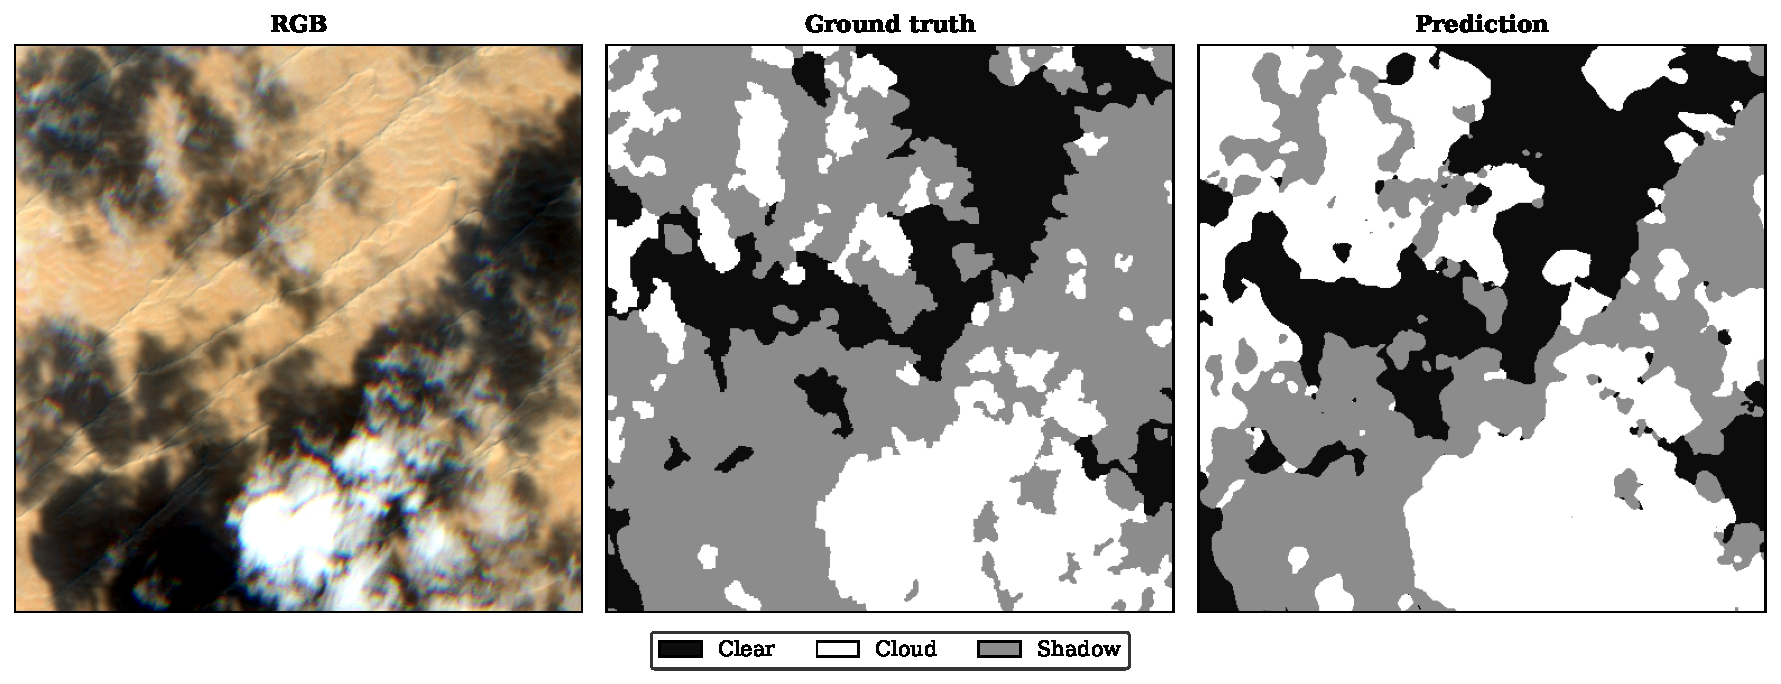
\includegraphics[width=\textwidth]{text/img/s2_vis/20190216T065941_20190216T070806_T39QVB_0_0_vis.pdf}
    \end{subfigure}
    \begin{subfigure}{\textwidth}
        \centering
        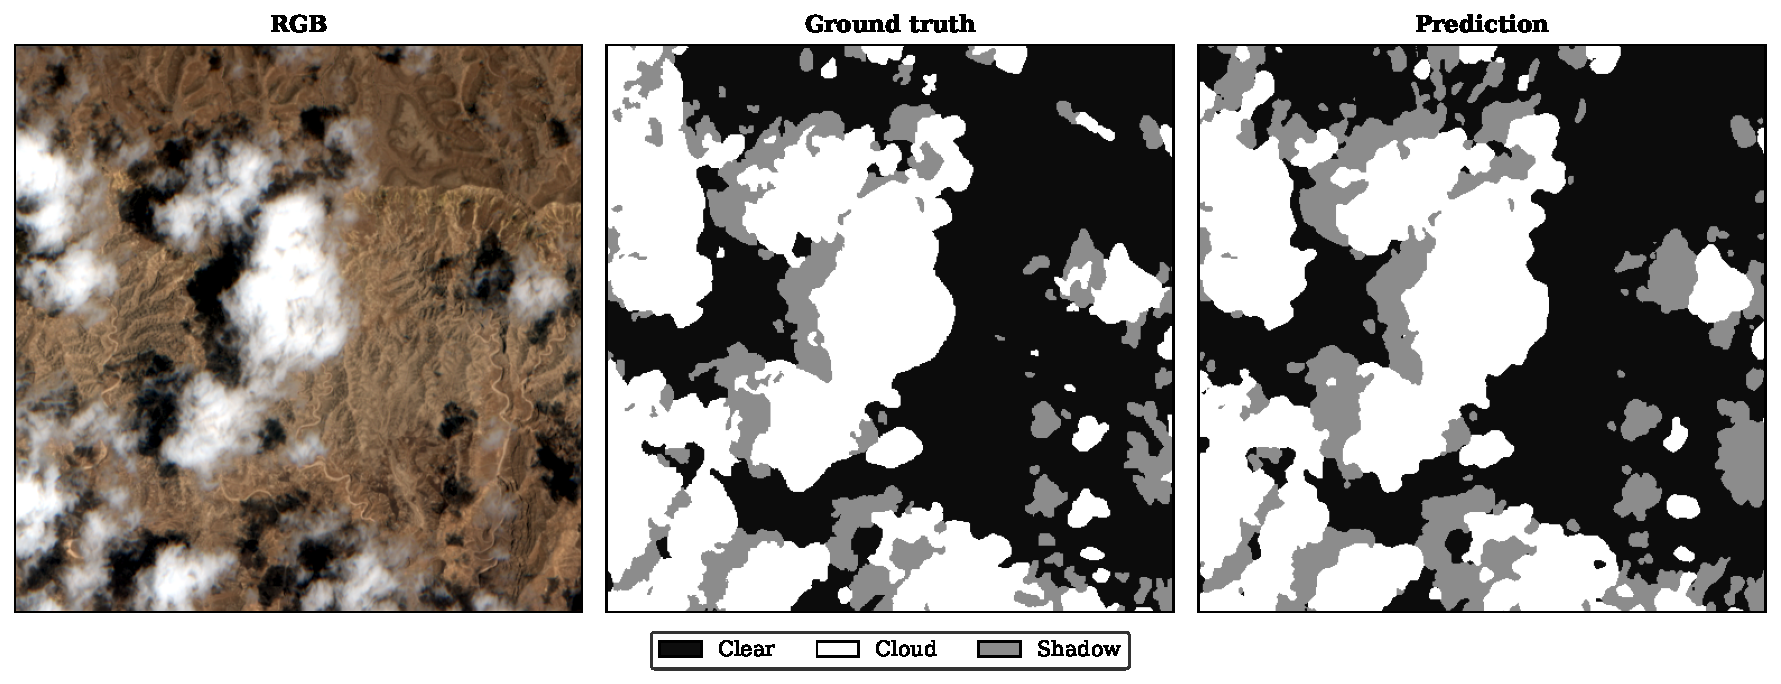
\includegraphics[width=\textwidth]{text/img/s2_vis/20190412T065629_20190412T070829_T39QXU_0_0_vis.pdf}
    \end{subfigure}
    \begin{subfigure}{\textwidth}
        \centering
        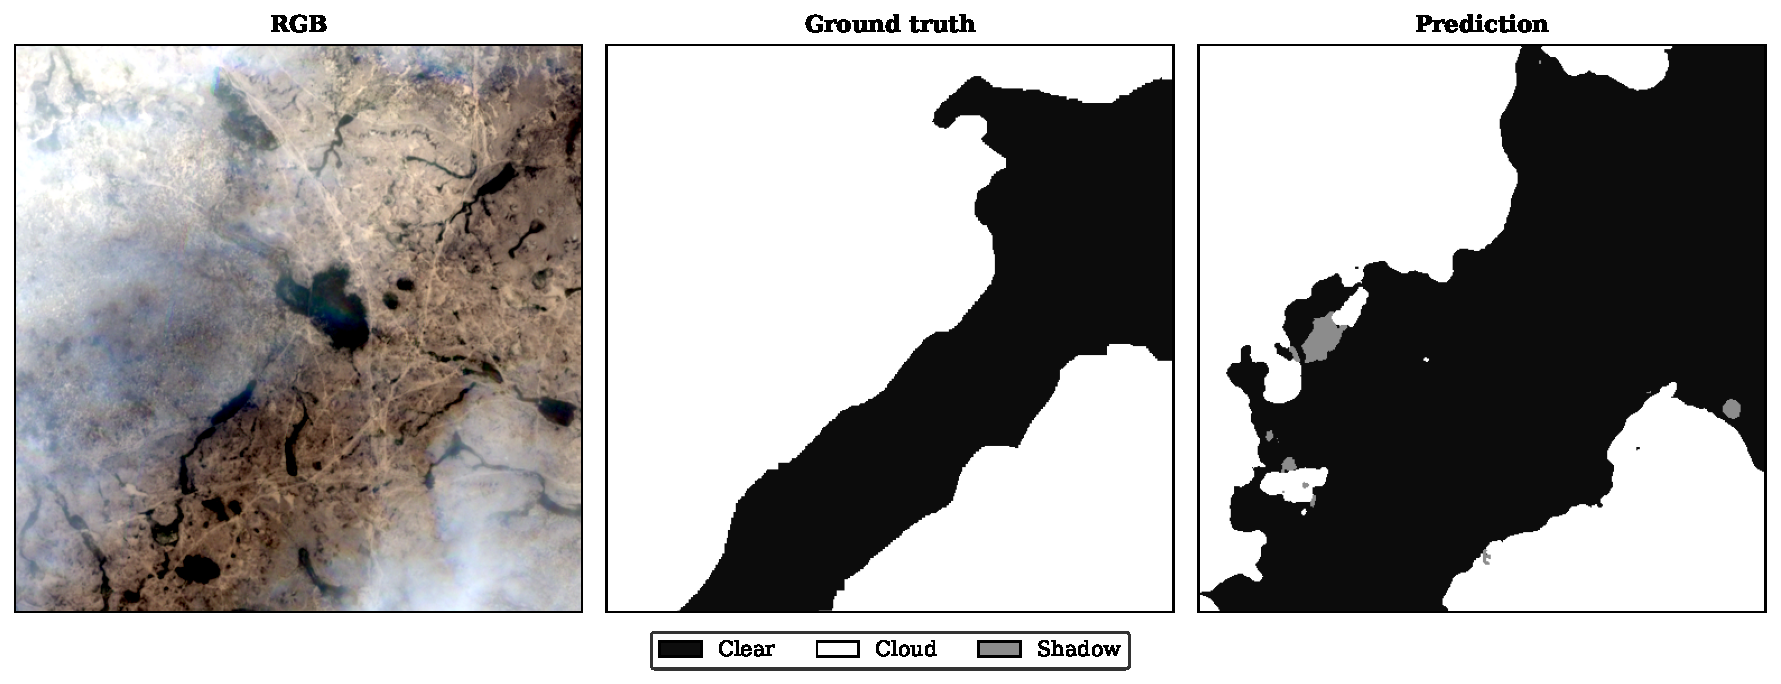
\includegraphics[width=\textwidth]{text/img/s2_vis/20190427T074619_20190427T075212_T37SGU_0_0_vis.pdf}
    \end{subfigure}
    \begin{subfigure}{\textwidth}
        \centering
        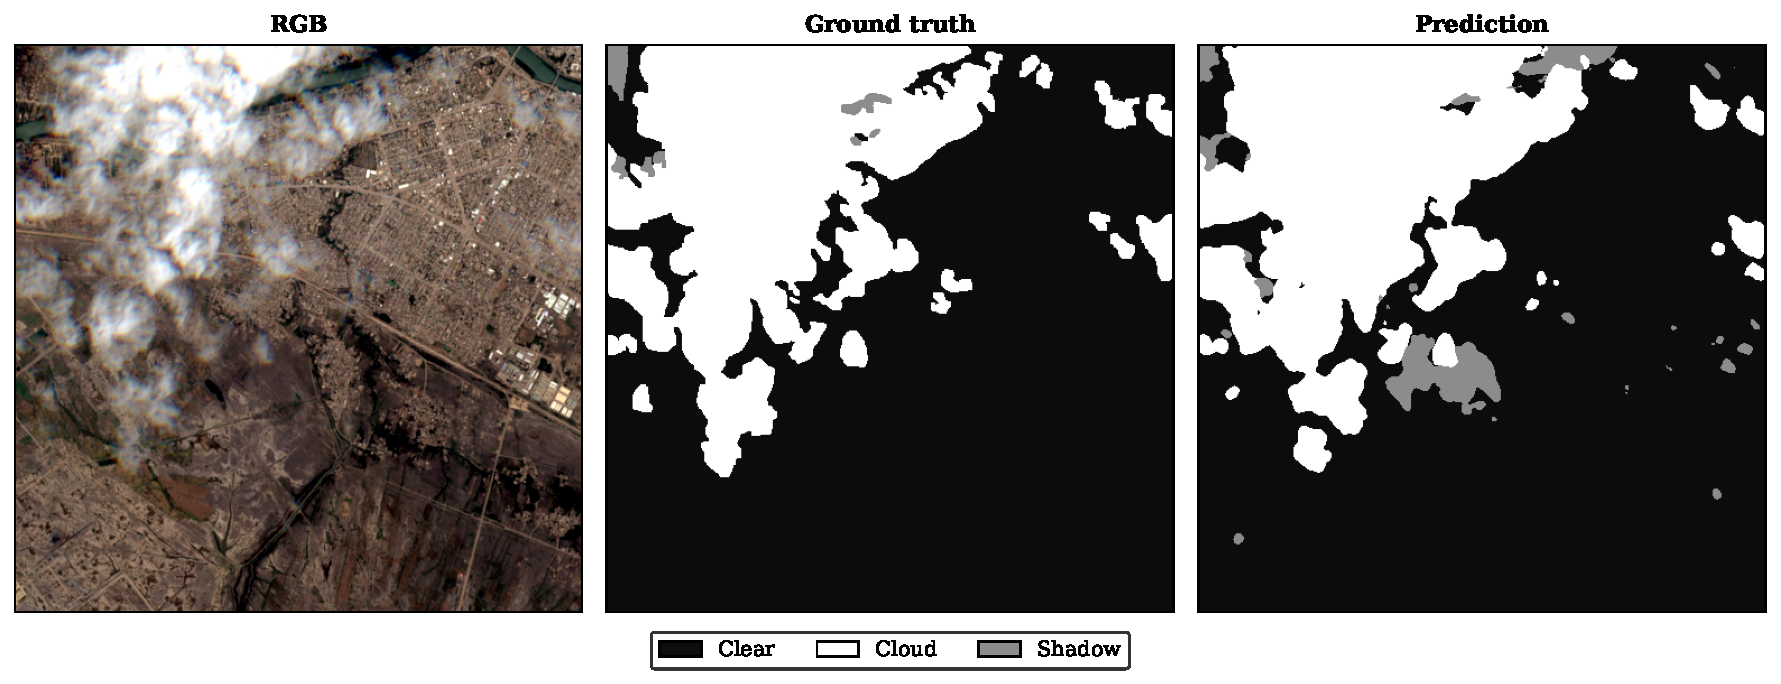
\includegraphics[width=\textwidth]{text/img/s2_vis/20190409T073611_20190409T074435_T38RPV_0_0_vis.pdf}
    \end{subfigure}
    \caption[Additional prediction examples for S2 model with dynamic Z-score 
    normalization.]{Additional prediction examples for the S2 model with dynamic 
    Z-score normalization on the S2 test set.}
    \label{fig:s2_visual_app}
\end{figure}

\section{VEN$\mu$S From Scratch}
\label{app:scratch}

\begin{figure}[H]
    \centering
    \begin{subfigure}{\textwidth}
        \centering
        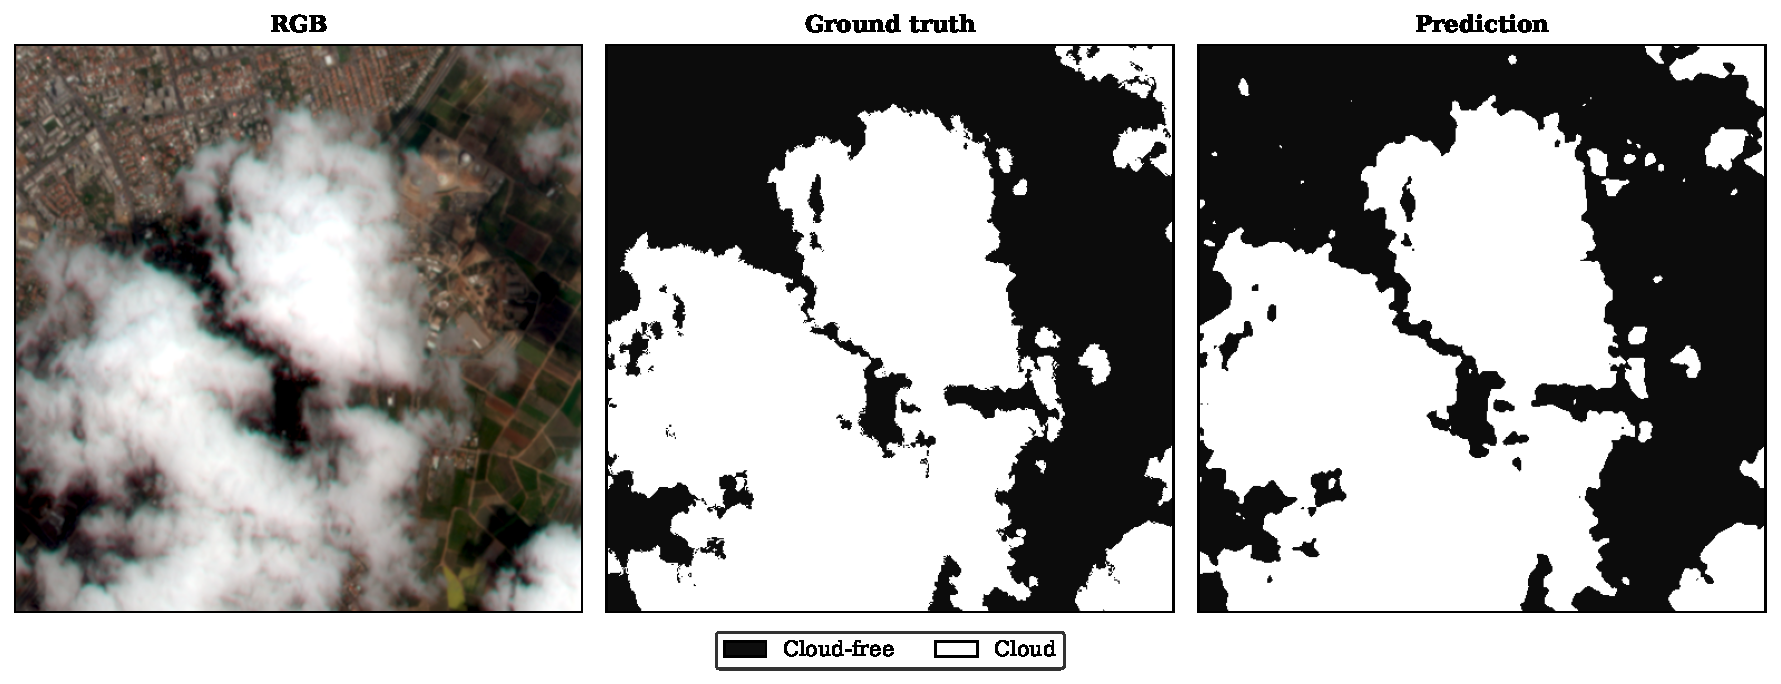
\includegraphics[width=0.98\textwidth]{text/img/venus_scratch_vis/s01_20190423_0_0_1536_1536_vis.pdf}
    \end{subfigure}
    \begin{subfigure}{\textwidth}
        \centering
        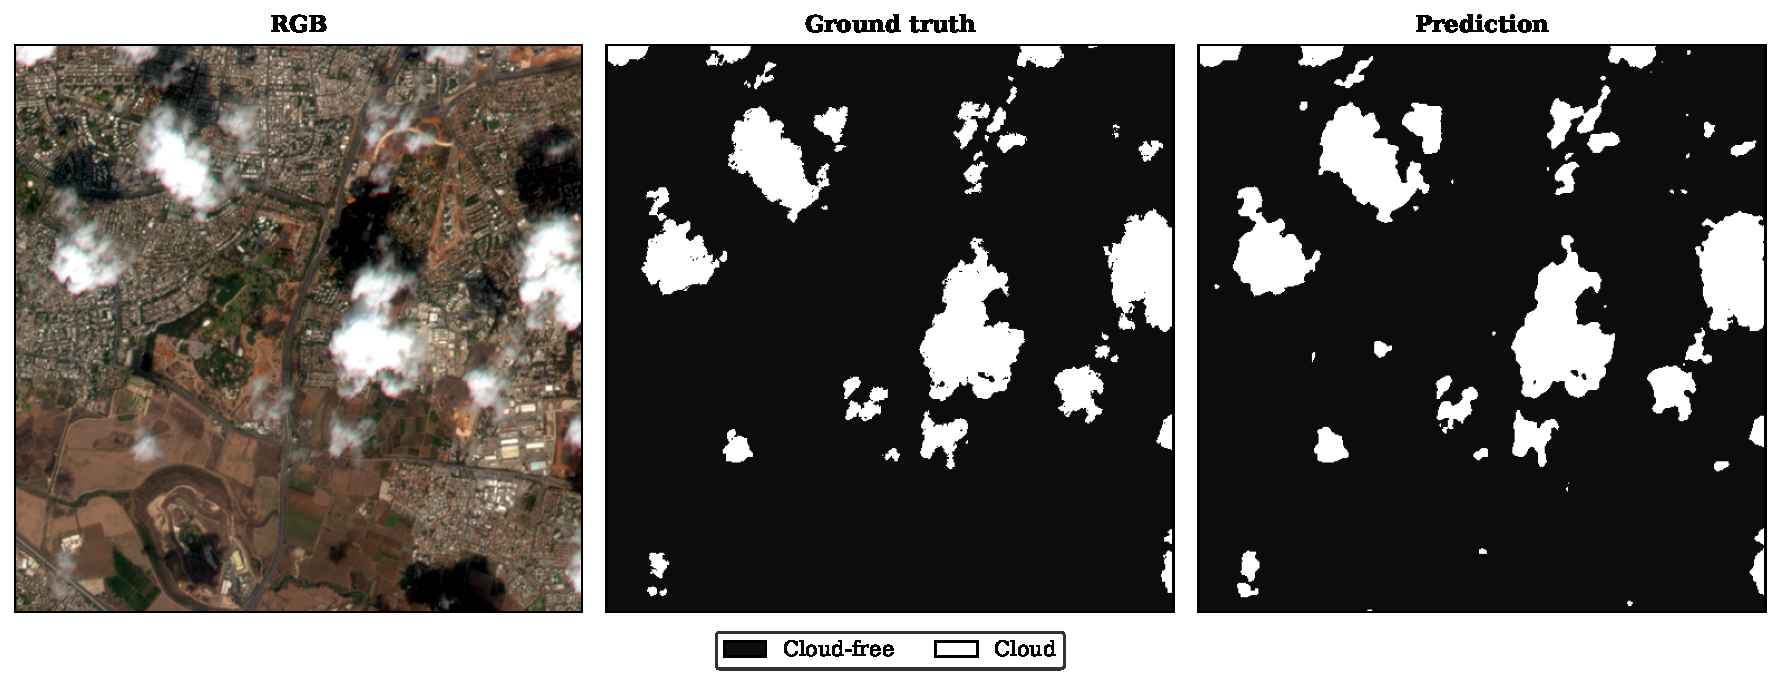
\includegraphics[width=0.98\textwidth]{text/img/venus_scratch_vis/w07_2048_0_0_1024_vis.pdf}
    \end{subfigure}
    \begin{subfigure}{\textwidth}
        \centering
        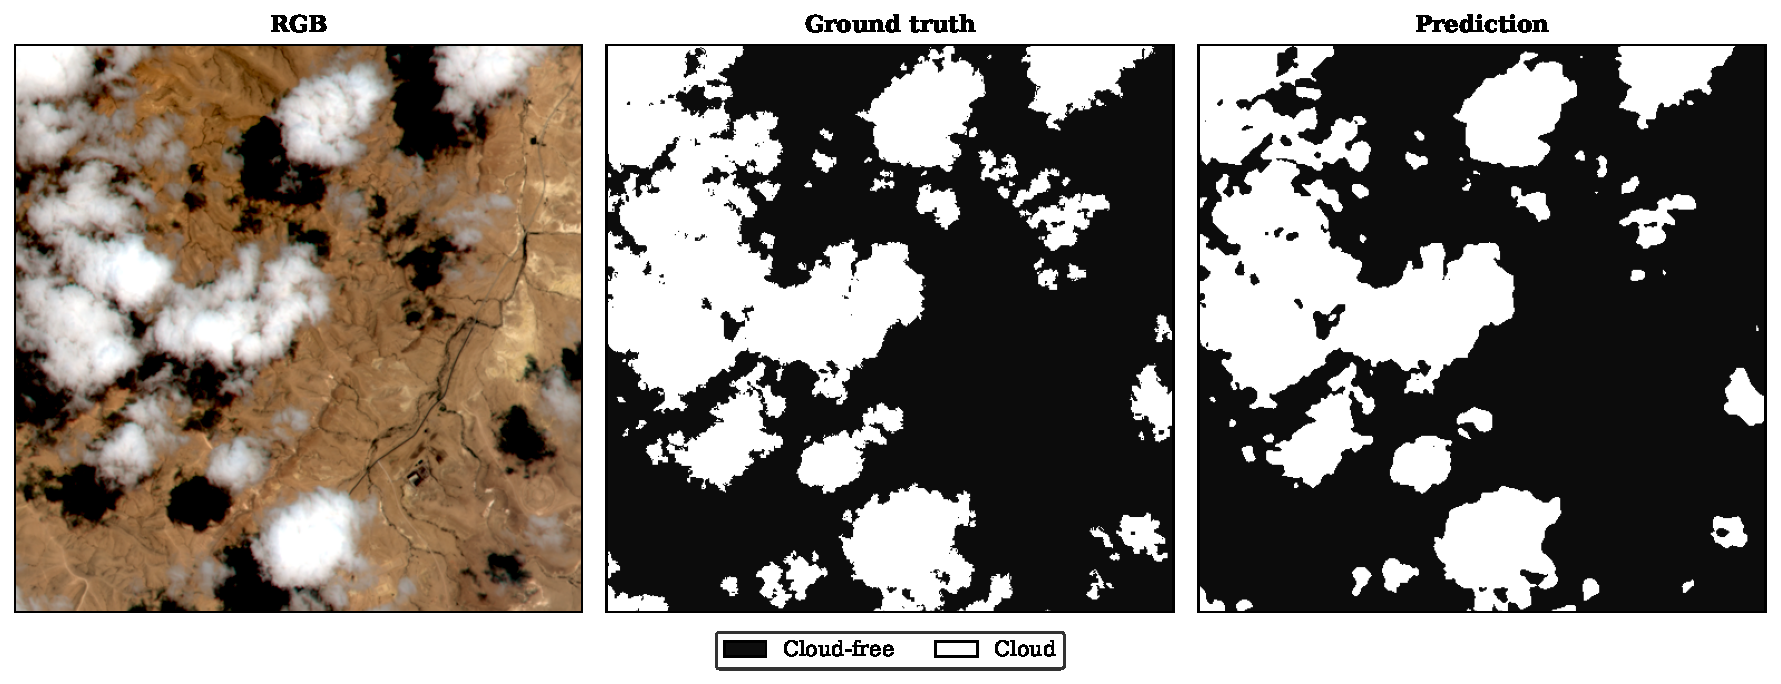
\includegraphics[width=0.98\textwidth]{text/img/venus_scratch_vis/s05_20180808_0_0_1024_0_vis.pdf}
    \end{subfigure}
    \begin{subfigure}{\textwidth}
        \centering
        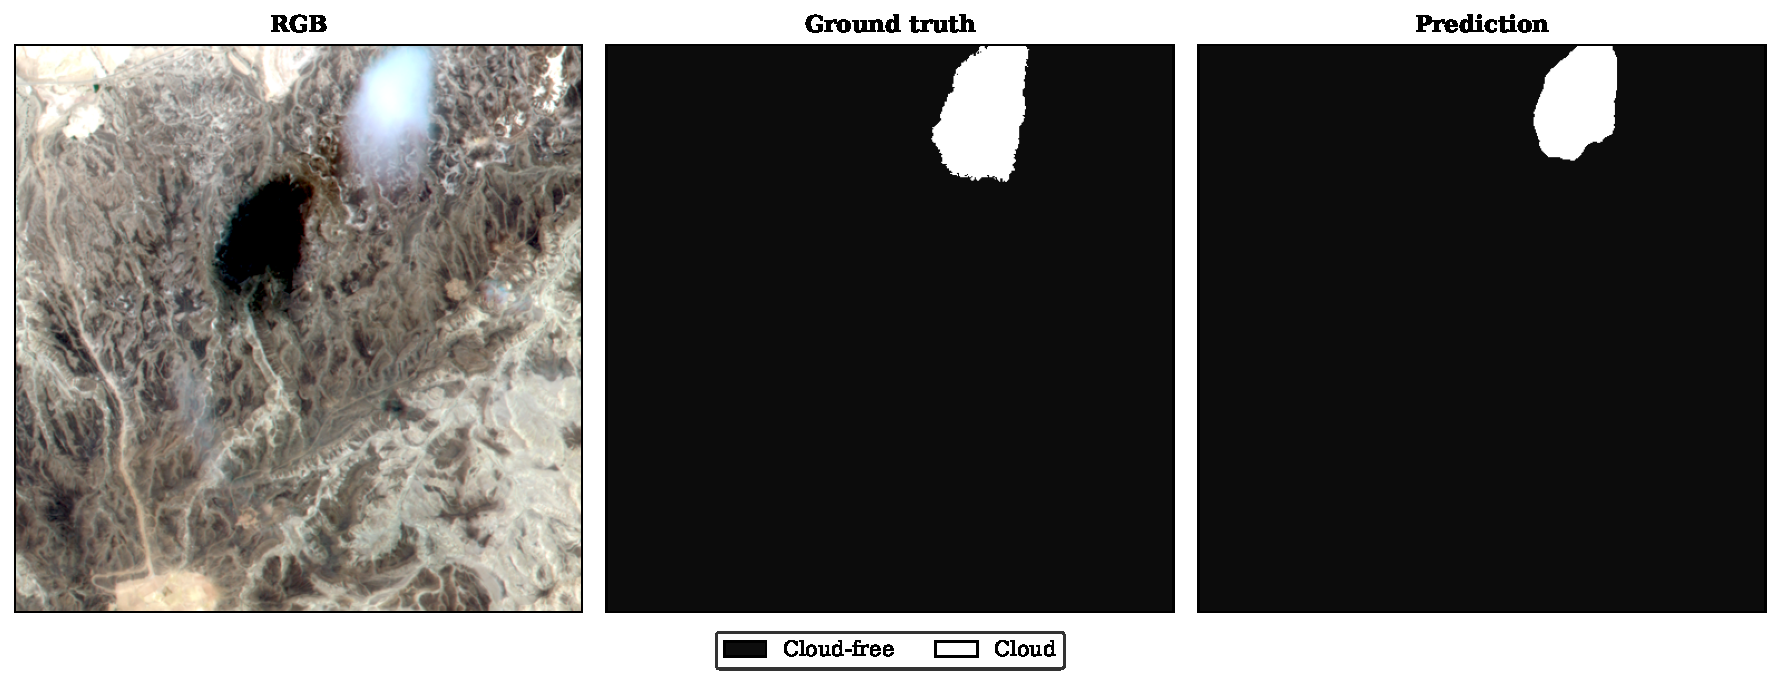
\includegraphics[width=0.98\textwidth]{text/img/venus_scratch_vis/s05_20180508_1793_1388_1024_512_vis.pdf}
    \end{subfigure}
    \caption[Additional prediction examples for VEN$\mu$S from-scratch model without normalization.]{Additional prediction examples for the VEN$\mu$S from-scratch model without normalization on the VEN$\mu$S test set.}
    \label{fig:scratch_visual_app}
\end{figure}


\section{Transductive Transfer Learning}
\label{app:transductive}

\begin{figure}[H]
    \centering
    \begin{subfigure}{\textwidth}
        \centering
        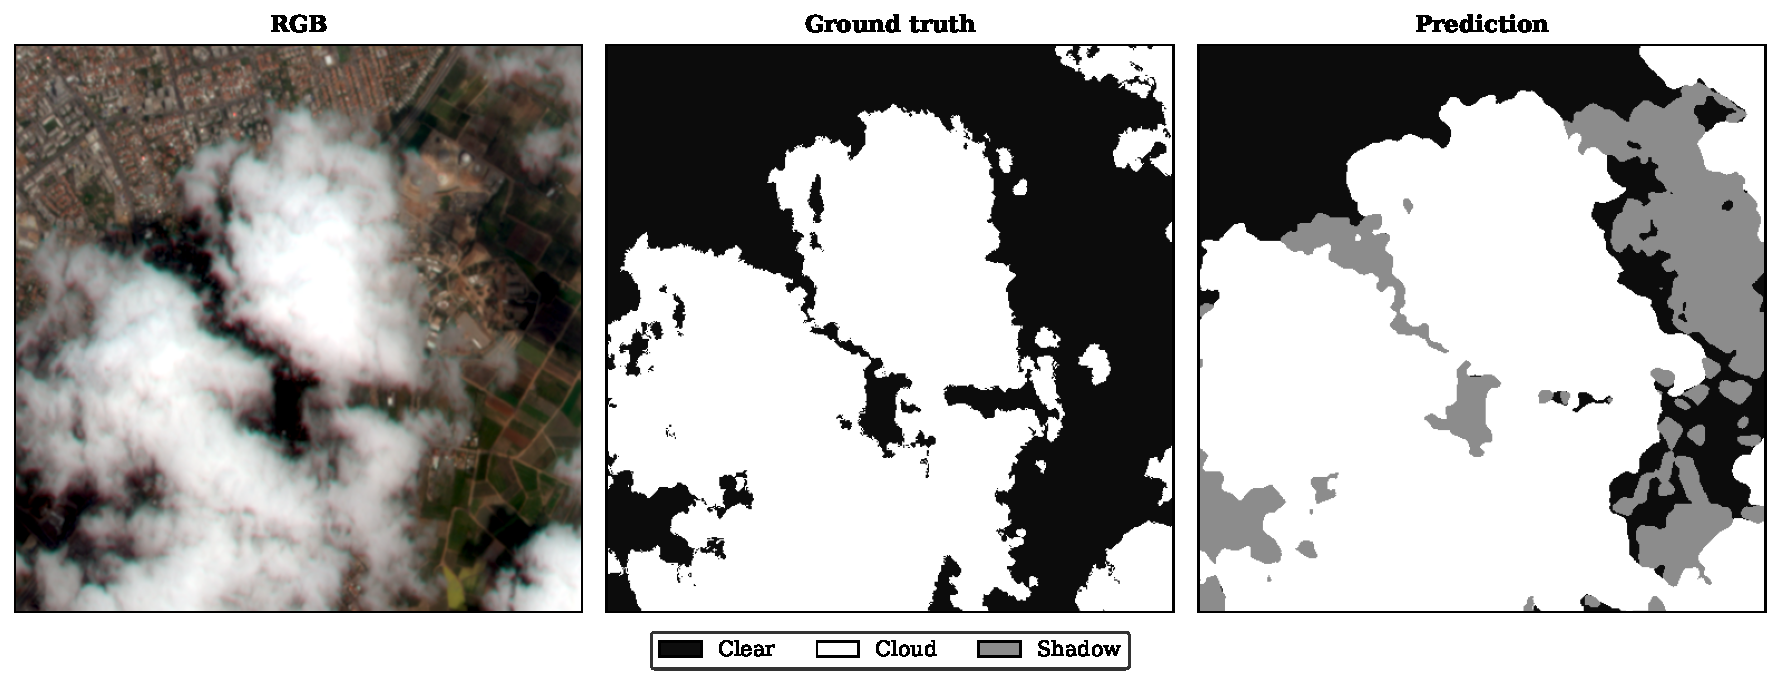
\includegraphics[width=0.98\textwidth]{text/img/e0_vis/s01_20190423_0_0_1536_1536_vis.pdf}
    \end{subfigure}
    \begin{subfigure}{\textwidth}
        \centering
        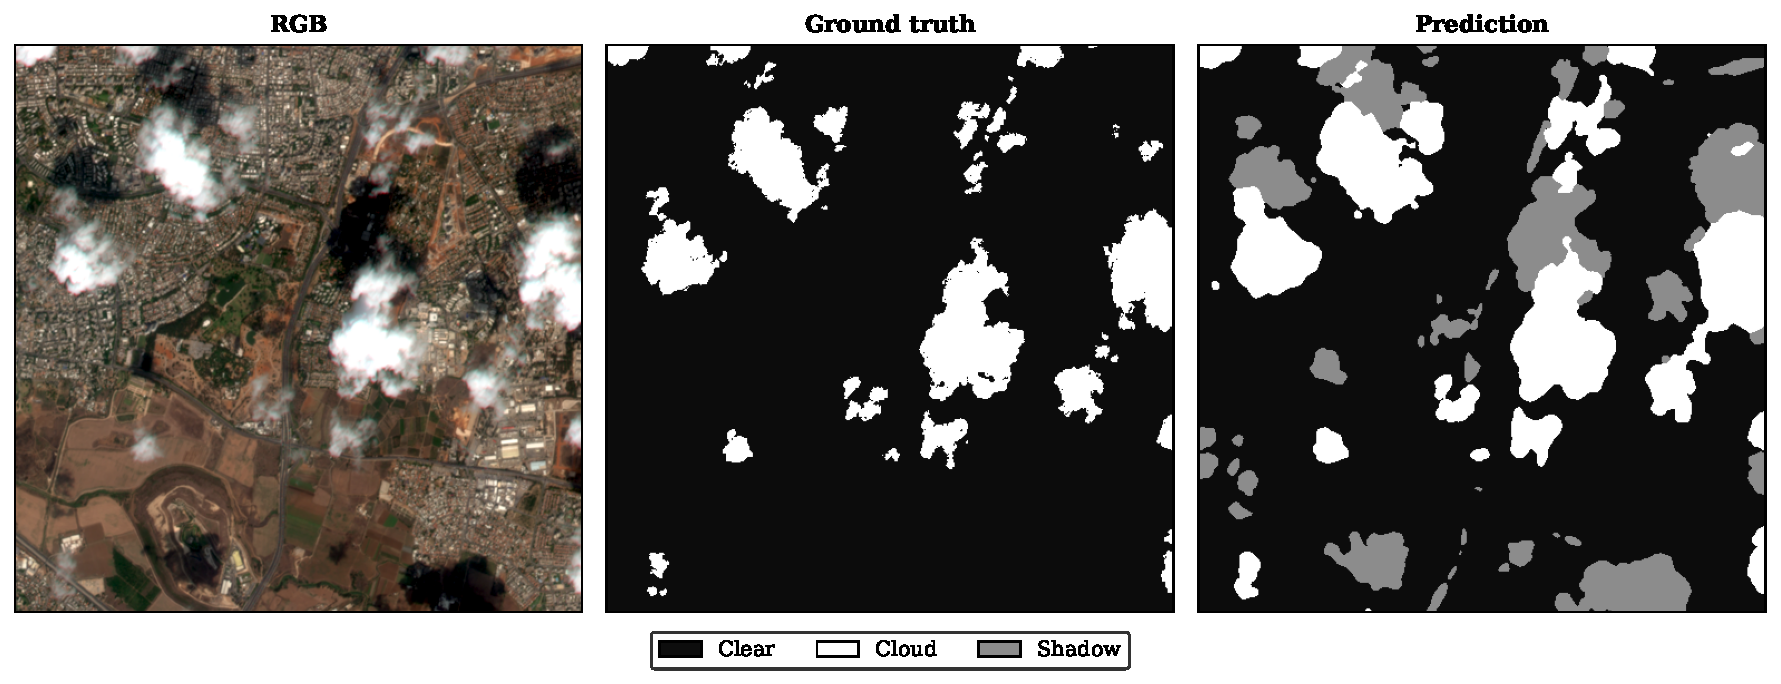
\includegraphics[width=0.98\textwidth]{text/img/e0_vis/w07_2048_0_0_1024_vis.pdf}
    \end{subfigure}
    \begin{subfigure}{\textwidth}
        \centering
        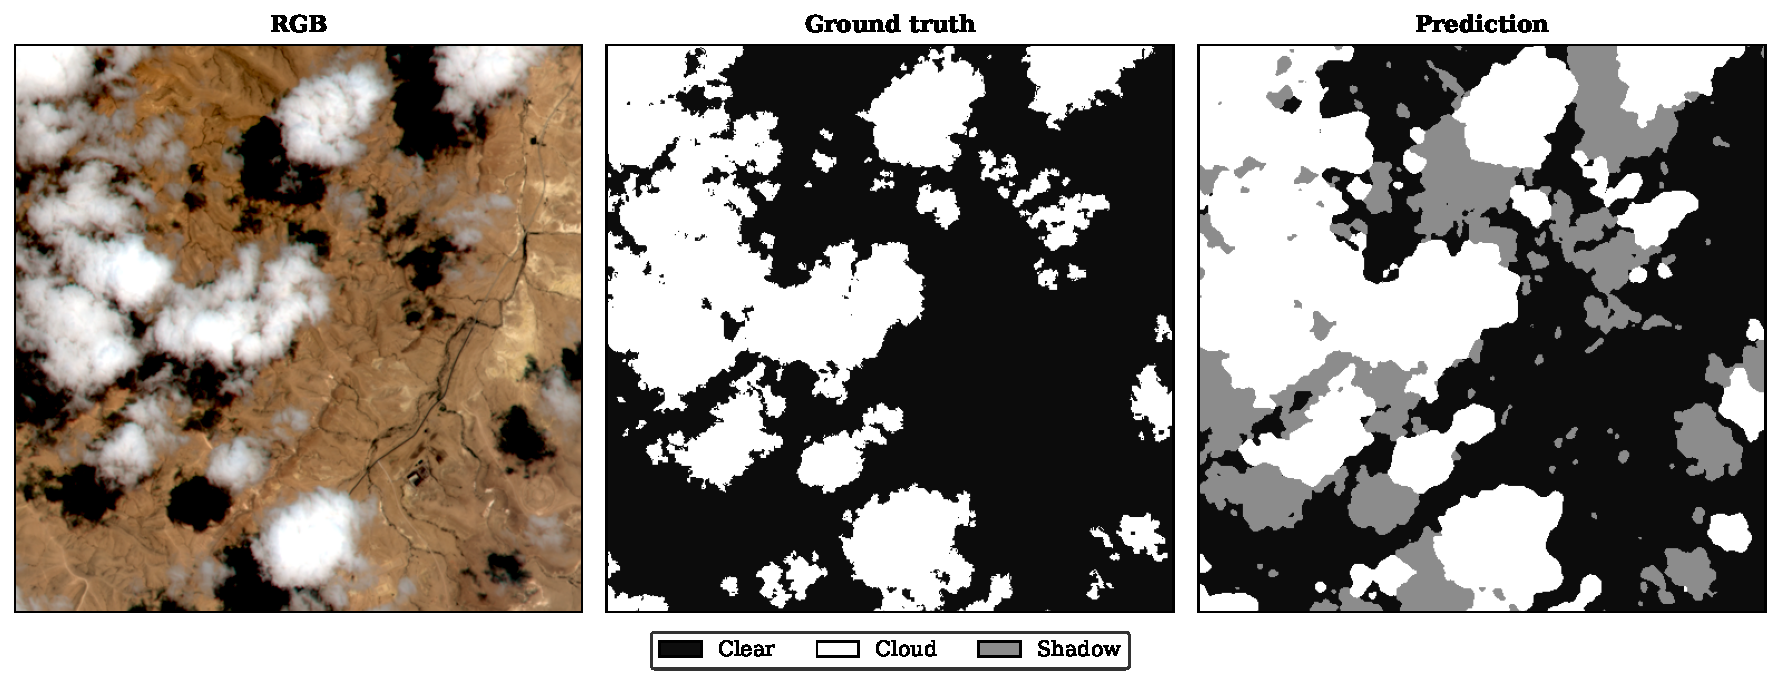
\includegraphics[width=0.98\textwidth]{text/img/e0_vis/s05_20180808_0_0_1024_0_vis.pdf}
    \end{subfigure}
    \begin{subfigure}{\textwidth}
        \centering
        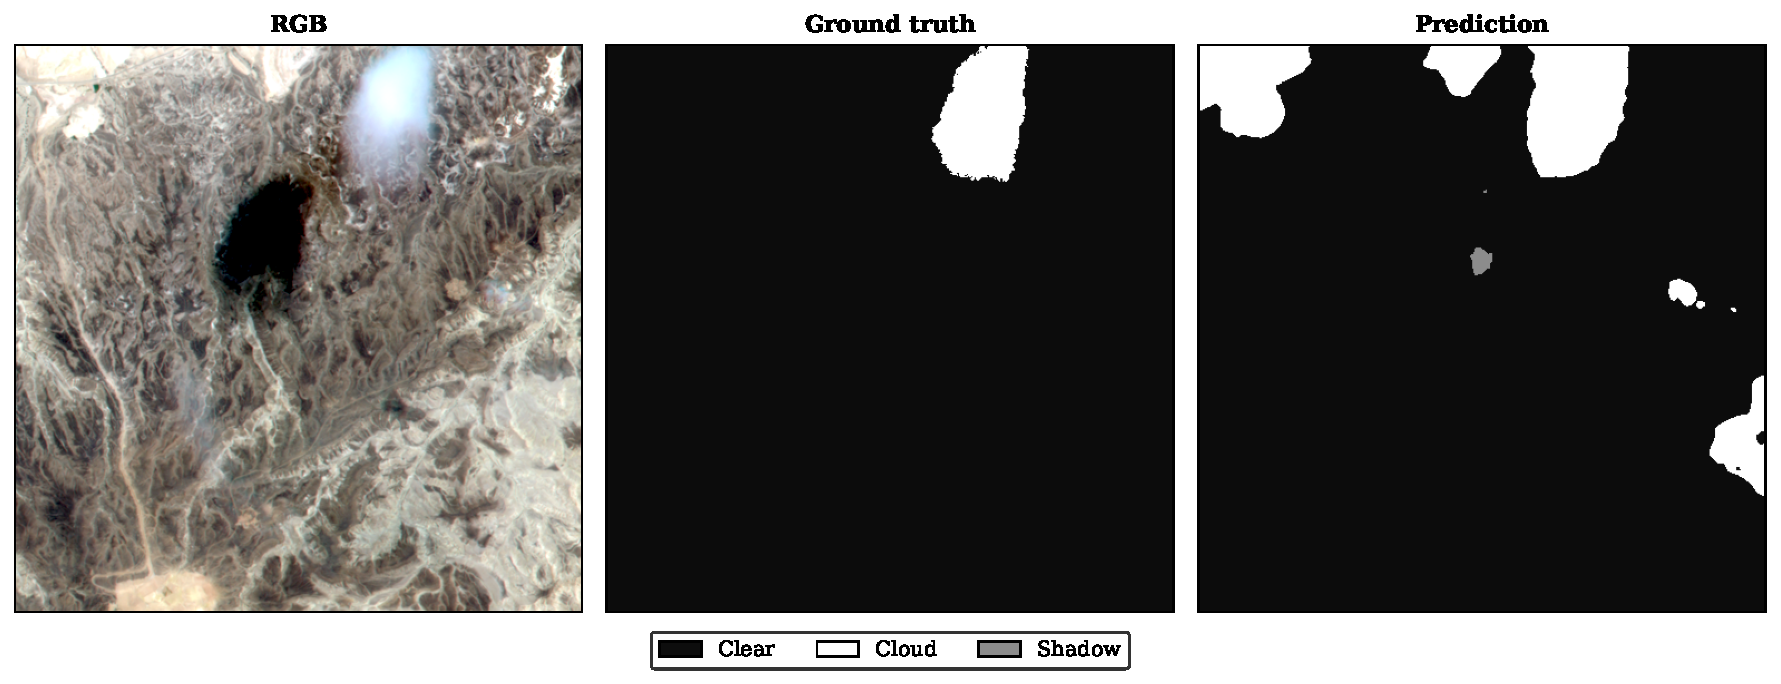
\includegraphics[width=0.98\textwidth]{text/img/e0_vis/s05_20180508_1793_1388_1024_512_vis.pdf}
    \end{subfigure}
    \caption[Additional prediction examples for transductive setting using dynamic Z-score normalization.]{Additional prediction examples for the transductive setting using dynamic Z-score normalization on the VEN$\mu$S test set.}
    \label{fig:e0_visual_app}
\end{figure}

\section{Output Layer Fine-Tuning}
\label{app:e1}

\begin{figure}[H]
    \centering
    \begin{subfigure}{\textwidth}
        \centering
        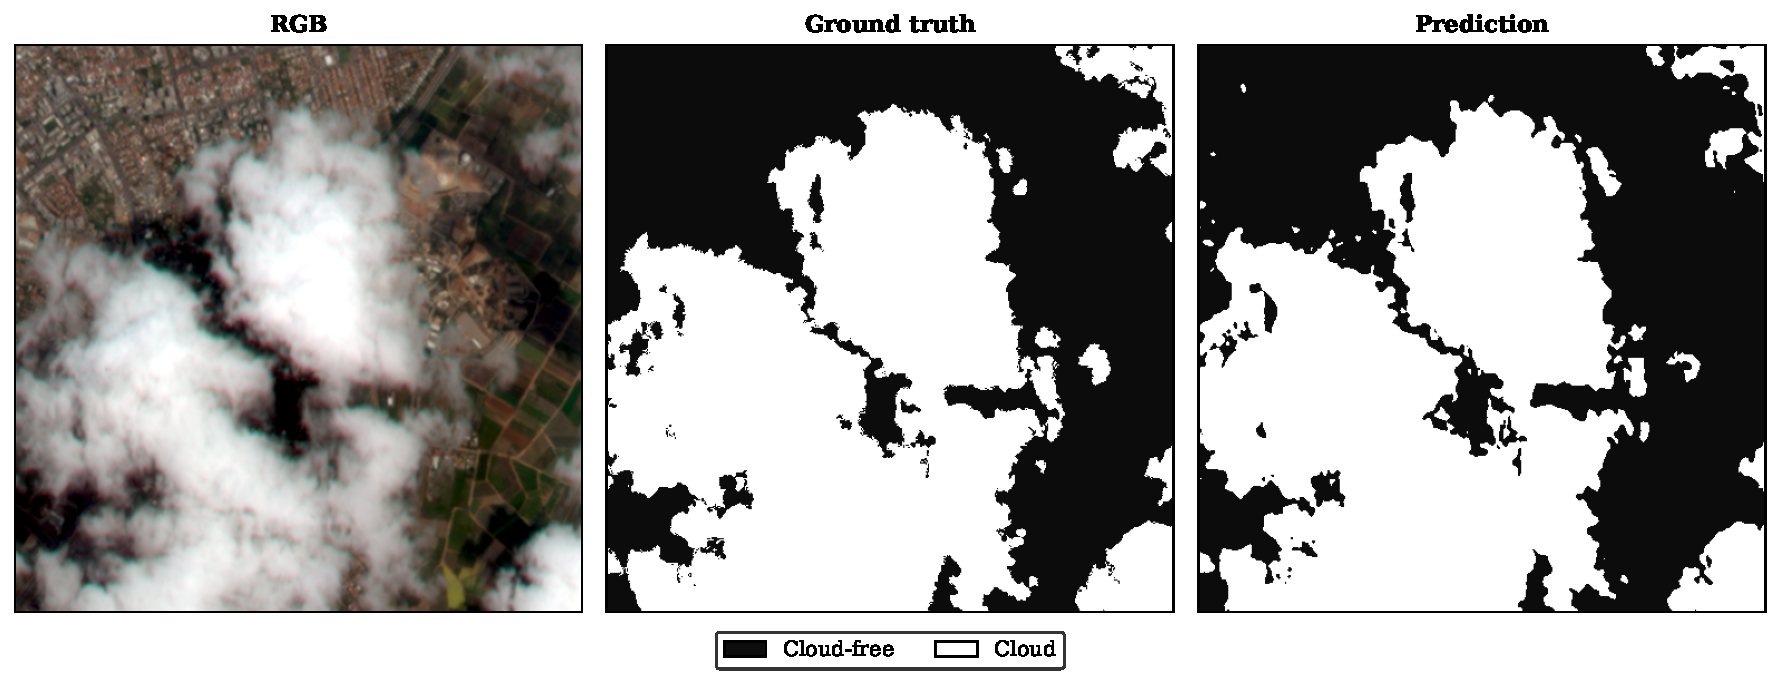
\includegraphics[width=0.98\textwidth]{text/img/e1_vis/s01_20190423_0_0_1536_1536_vis.pdf}
    \end{subfigure}
    \begin{subfigure}{\textwidth}
        \centering
        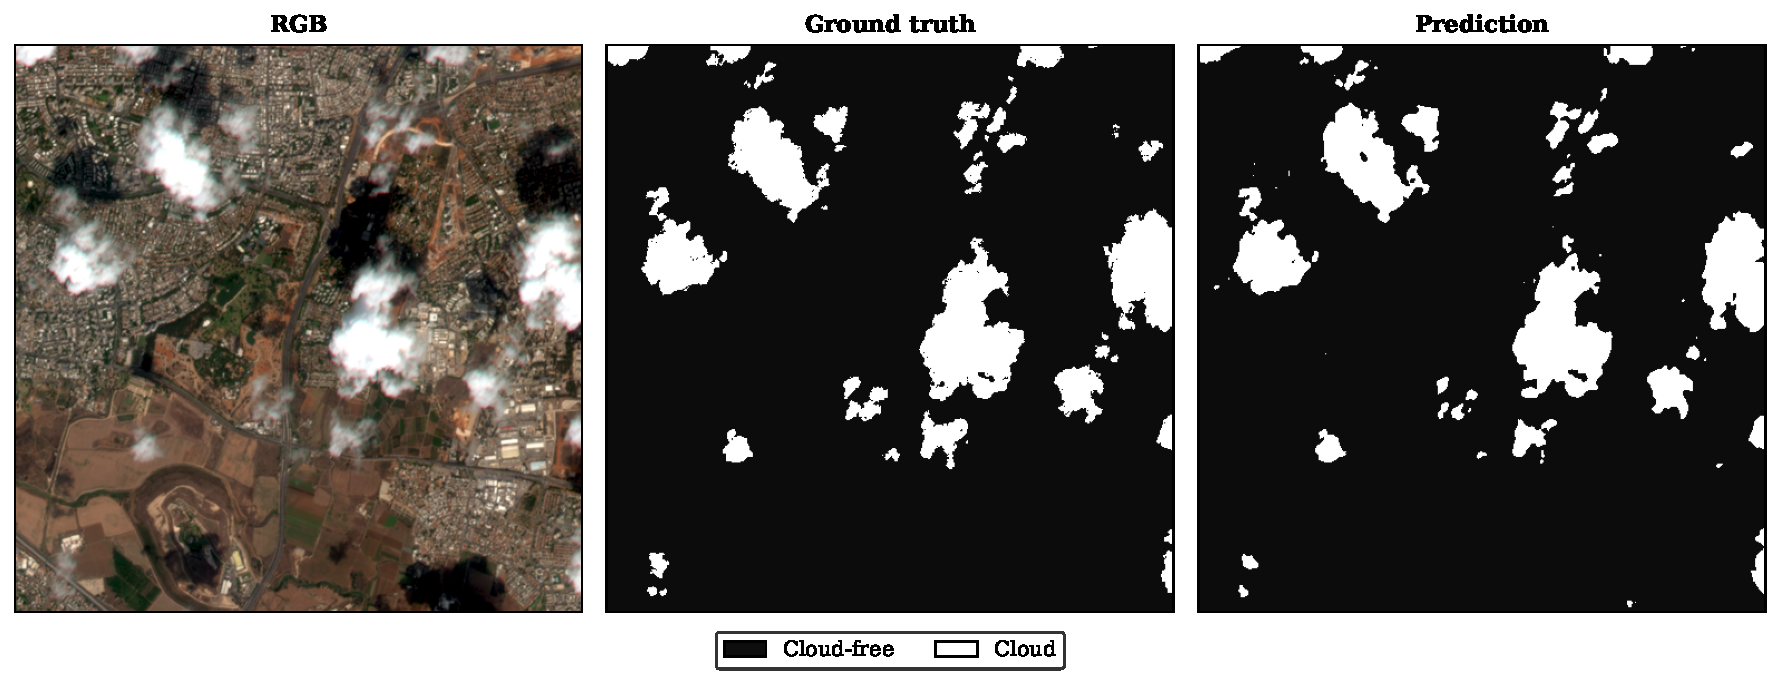
\includegraphics[width=0.98\textwidth]{text/img/e1_vis/w07_2048_0_0_1024_vis.pdf}
    \end{subfigure}
    \begin{subfigure}{\textwidth}
        \centering
        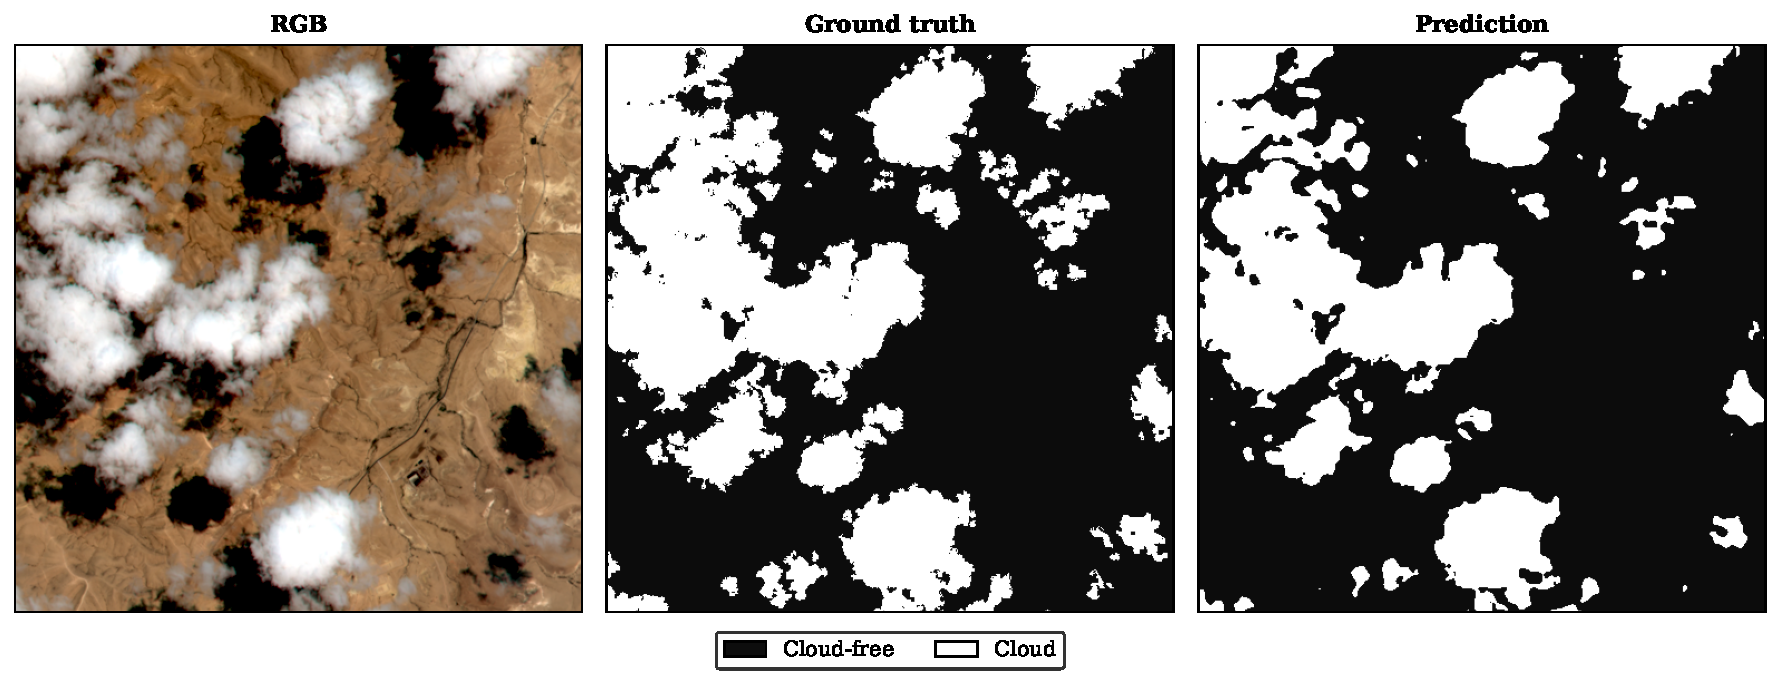
\includegraphics[width=0.98\textwidth]{text/img/e1_vis/s05_20180808_0_0_1024_0_vis.pdf}
    \end{subfigure}
    \begin{subfigure}{\textwidth}
        \centering
        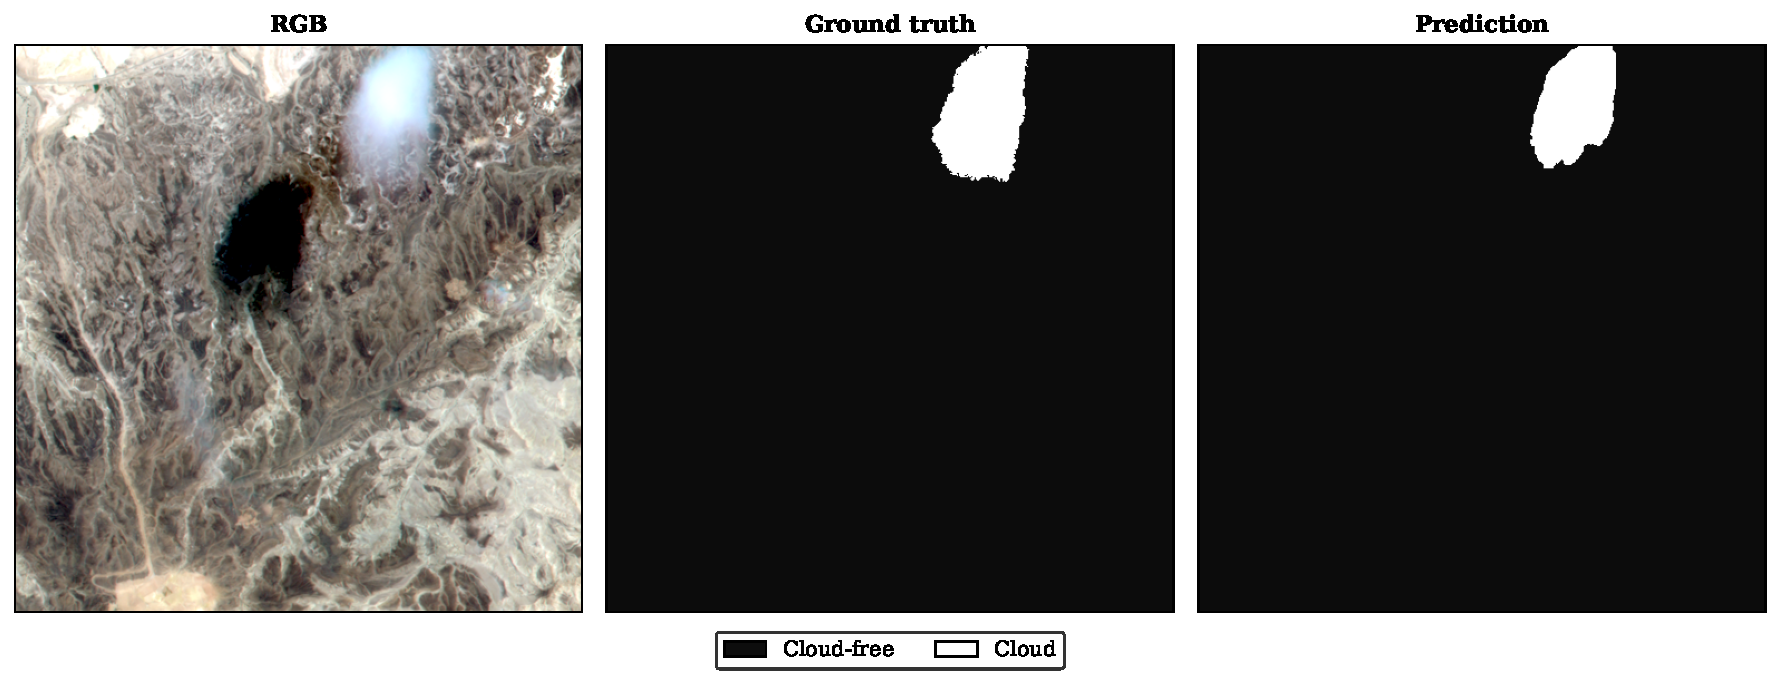
\includegraphics[width=0.98\textwidth]{text/img/e1_vis/s05_20180508_1793_1388_1024_512_vis.pdf}
    \end{subfigure}
    \caption[Additional prediction examples for output layer fine-tuning using fixed Z-score normalization with VEN$\mu$S statistics.]{Additional prediction examples for output layer fine-tuning using fixed Z-score normalization with VEN$\mu$S statistics on the VEN$\mu$S test set.}
    \label{fig:e1_visual_app}
\end{figure}

\section{Frozen Encoder Fine-Tuning}
\label{app:e2}

\begin{figure}[H]
    \centering
    \begin{subfigure}{\textwidth}
        \centering
        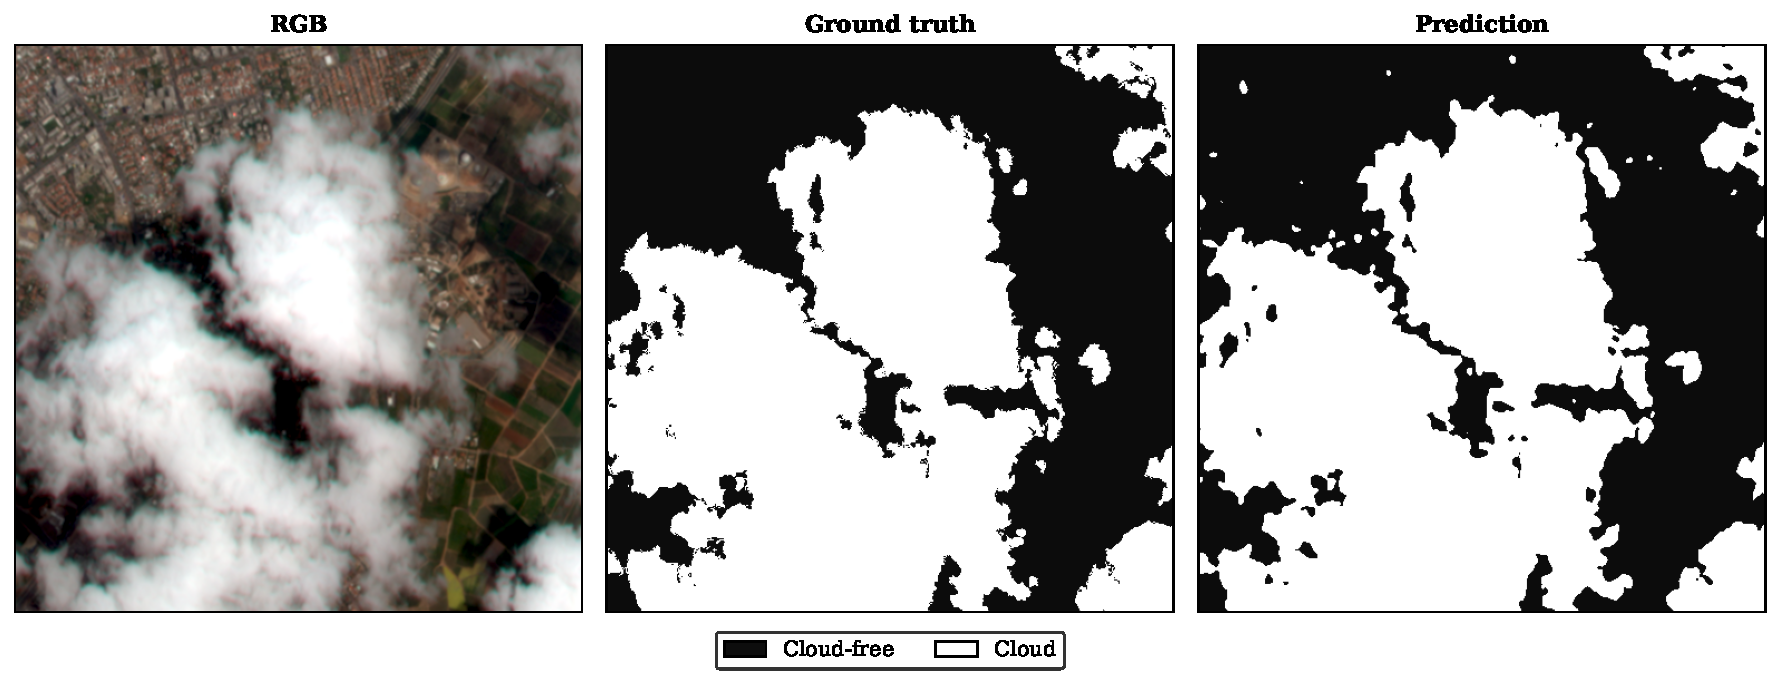
\includegraphics[width=0.98\textwidth]{text/img/e2_vis/s01_20190423_0_0_1536_1536_vis.pdf}
    \end{subfigure}
    \begin{subfigure}{\textwidth}
        \centering
        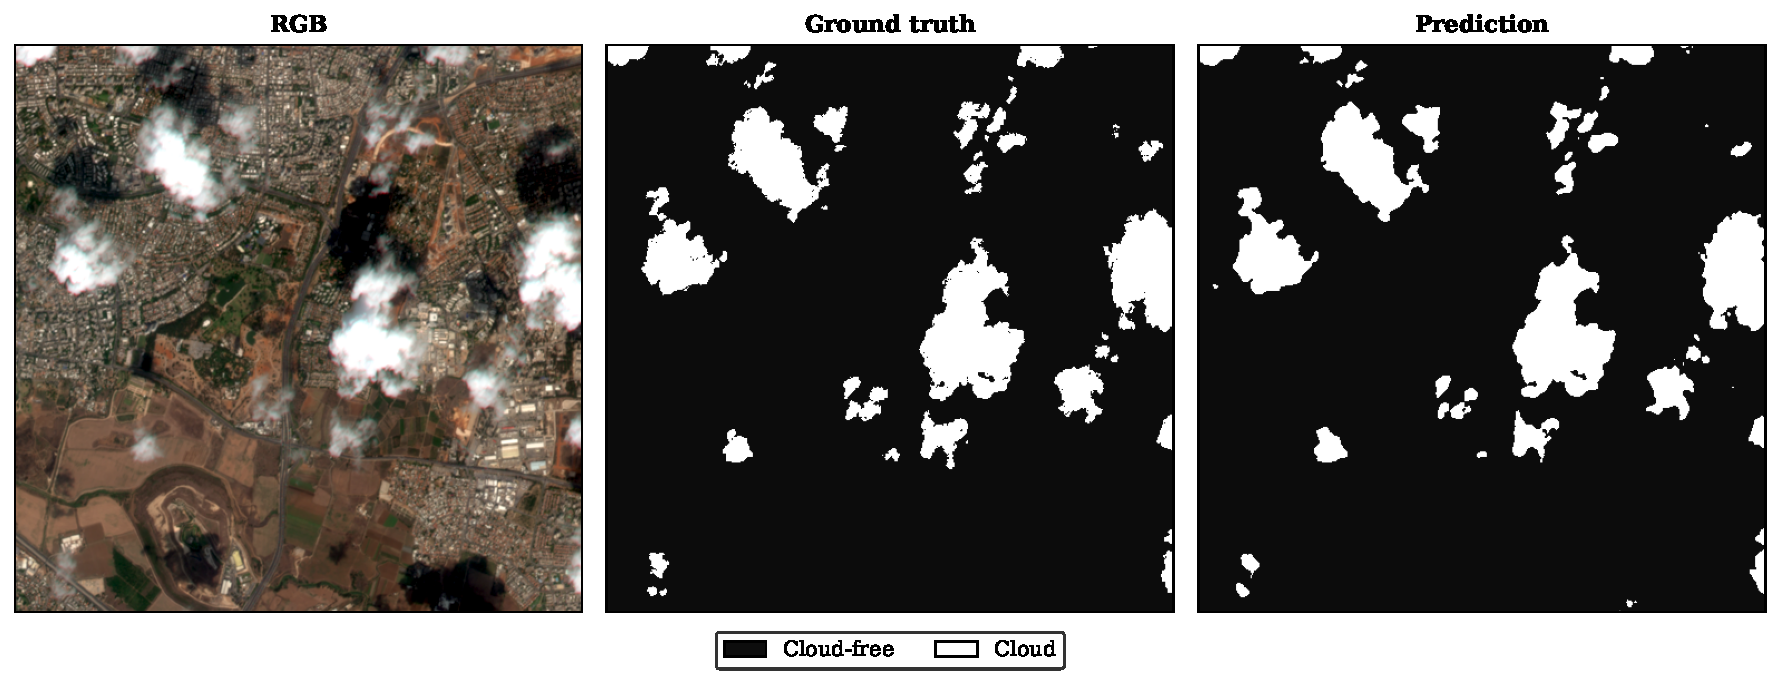
\includegraphics[width=0.98\textwidth]{text/img/e2_vis/w07_2048_0_0_1024_vis.pdf}
    \end{subfigure}
    \begin{subfigure}{\textwidth}
        \centering
        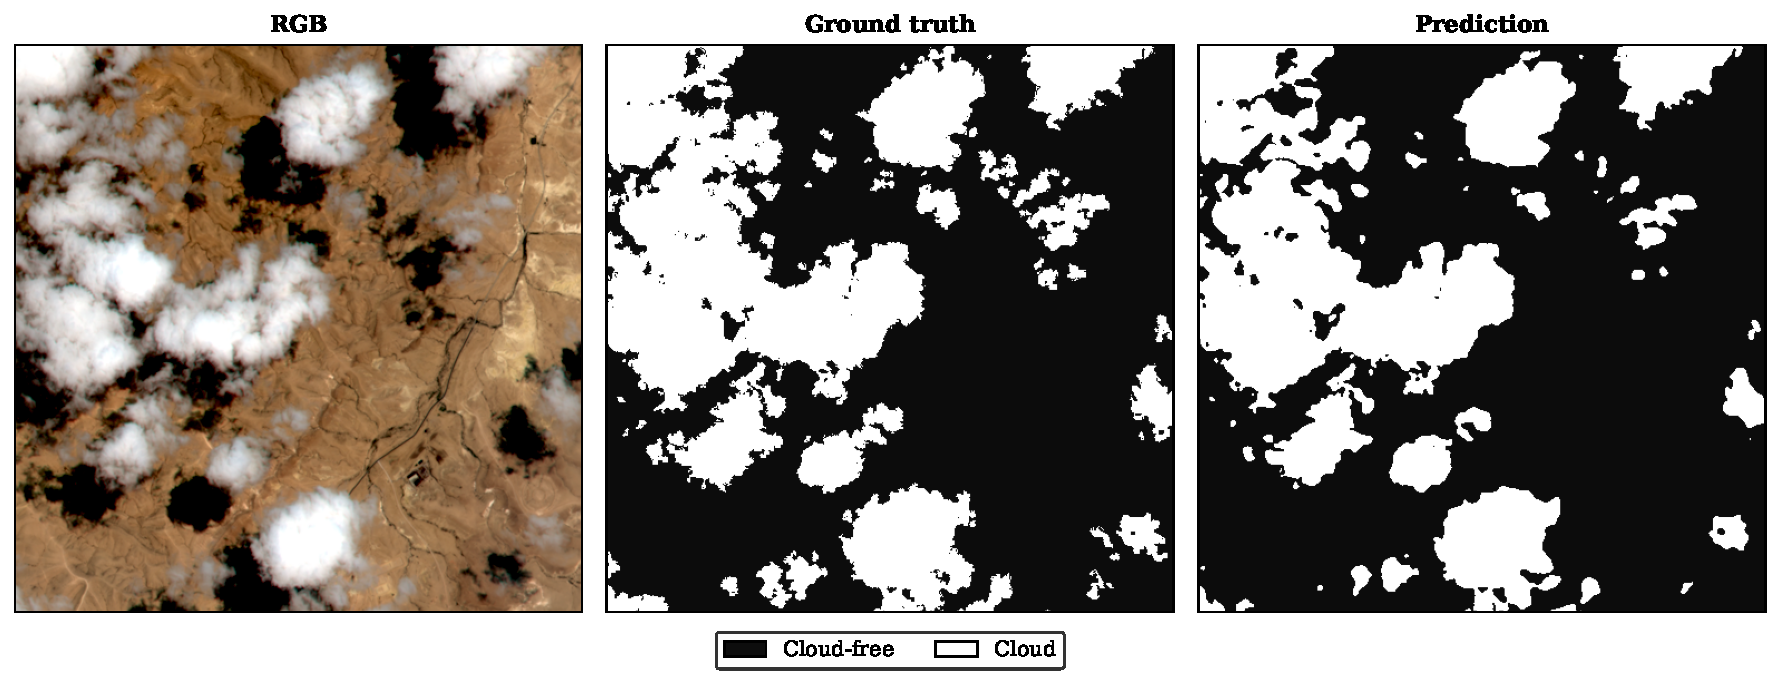
\includegraphics[width=0.98\textwidth]{text/img/e2_vis/s05_20180808_0_0_1024_0_vis.pdf}
    \end{subfigure}
    \begin{subfigure}{\textwidth}
        \centering
        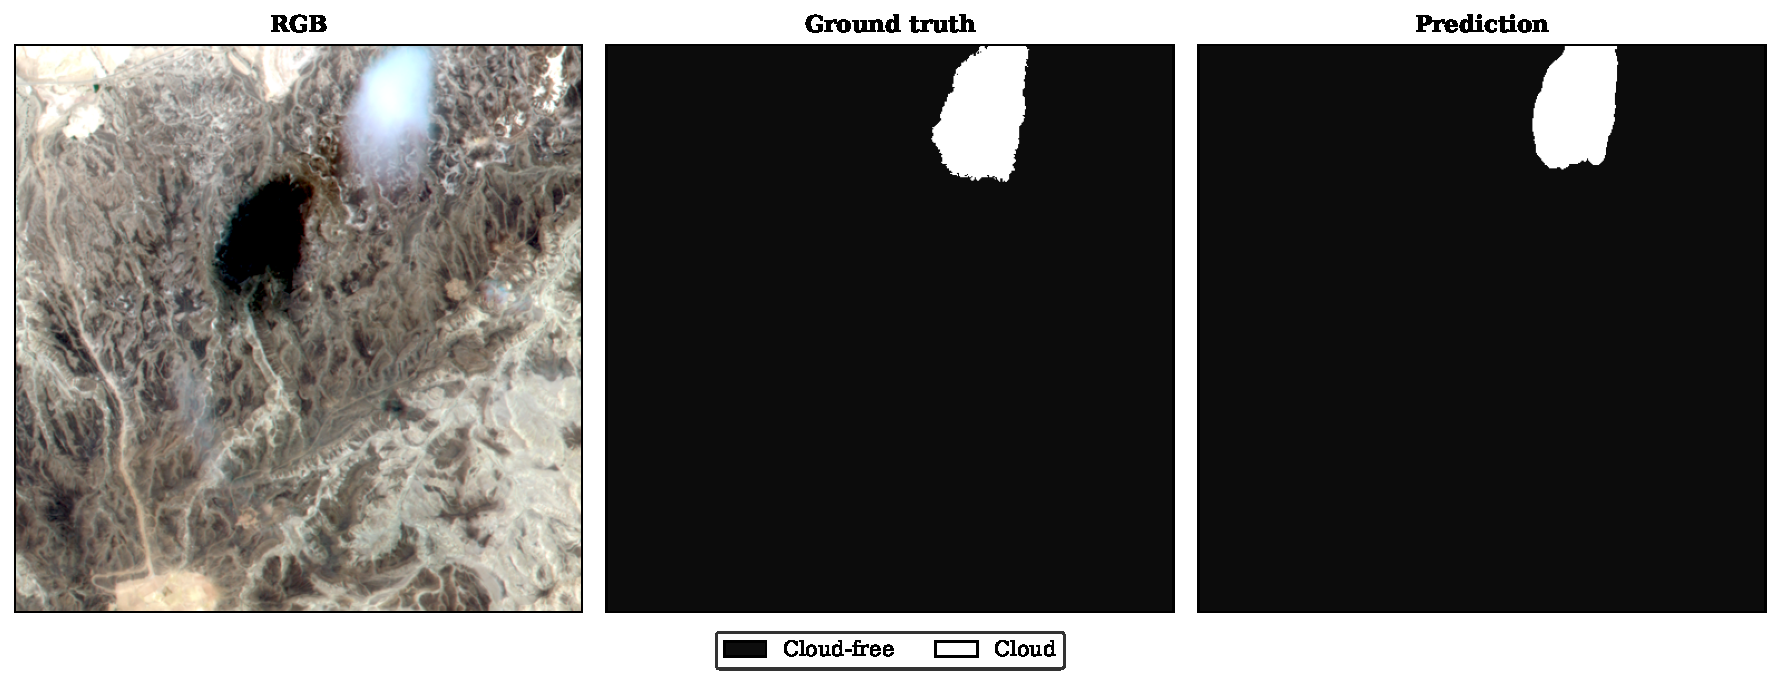
\includegraphics[width=0.98\textwidth]{text/img/e2_vis/s05_20180508_1793_1388_1024_512_vis.pdf}
    \end{subfigure}
    \caption[Additional prediction examples for frozen encoder fine-tuning using fixed Z-score normalization with VEN$\mu$S statistics.]{Additional prediction examples for frozen encoder fine-tuning with fixed Z-score normalization with VEN$\mu$S statistics on the VEN$\mu$S test set.}
    \label{fig:e2_visual_app}
\end{figure}

\section{Full Fine-Tuning}
\label{app:e3}

\begin{figure}[H]
    \centering
    \begin{subfigure}{\textwidth}
        \centering
        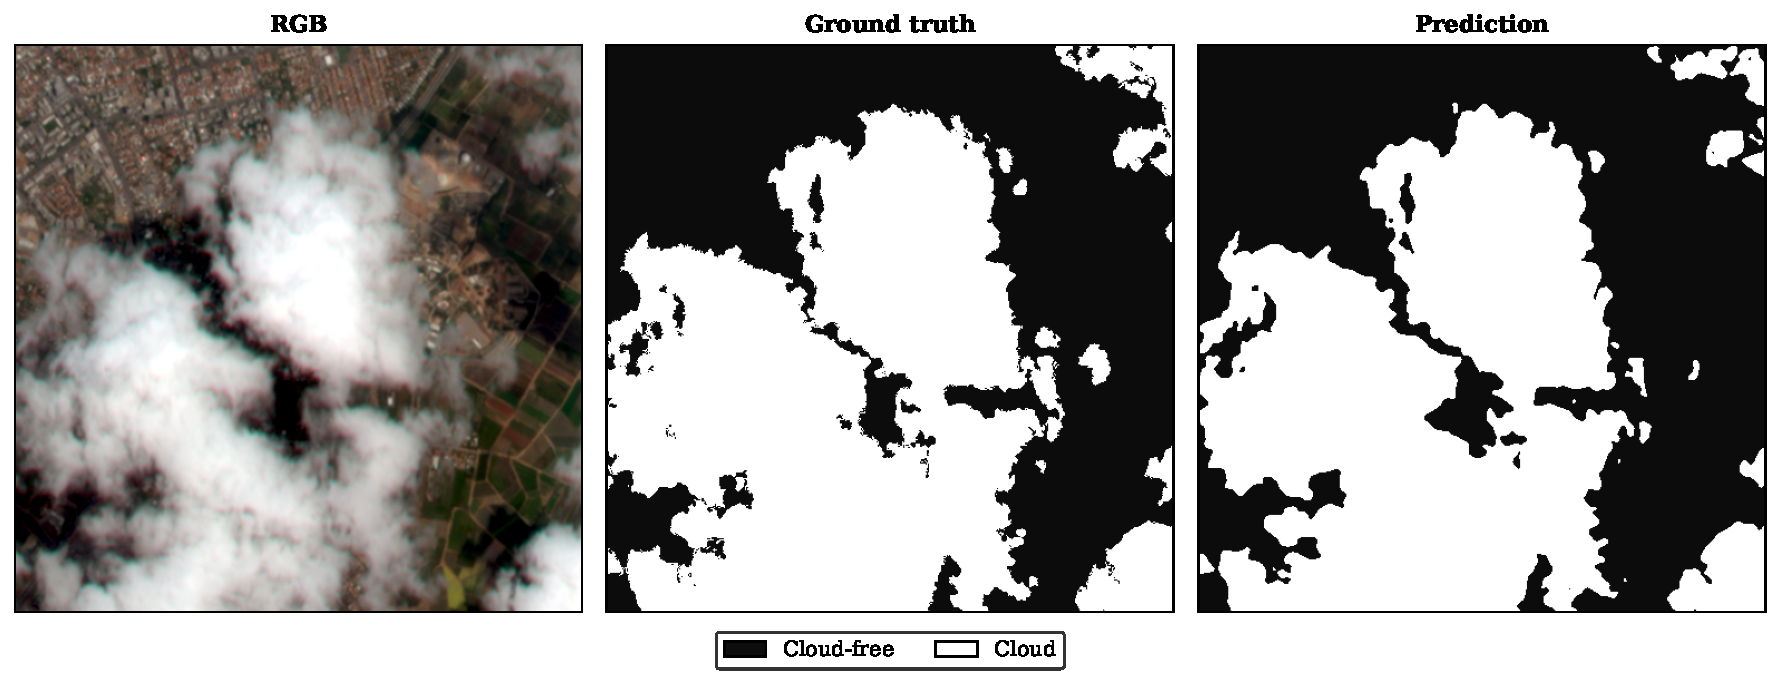
\includegraphics[width=0.98\textwidth]{text/img/e3_vis/s01_20190423_0_0_1536_1536_vis.pdf}
    \end{subfigure}
    \begin{subfigure}{\textwidth}
        \centering
        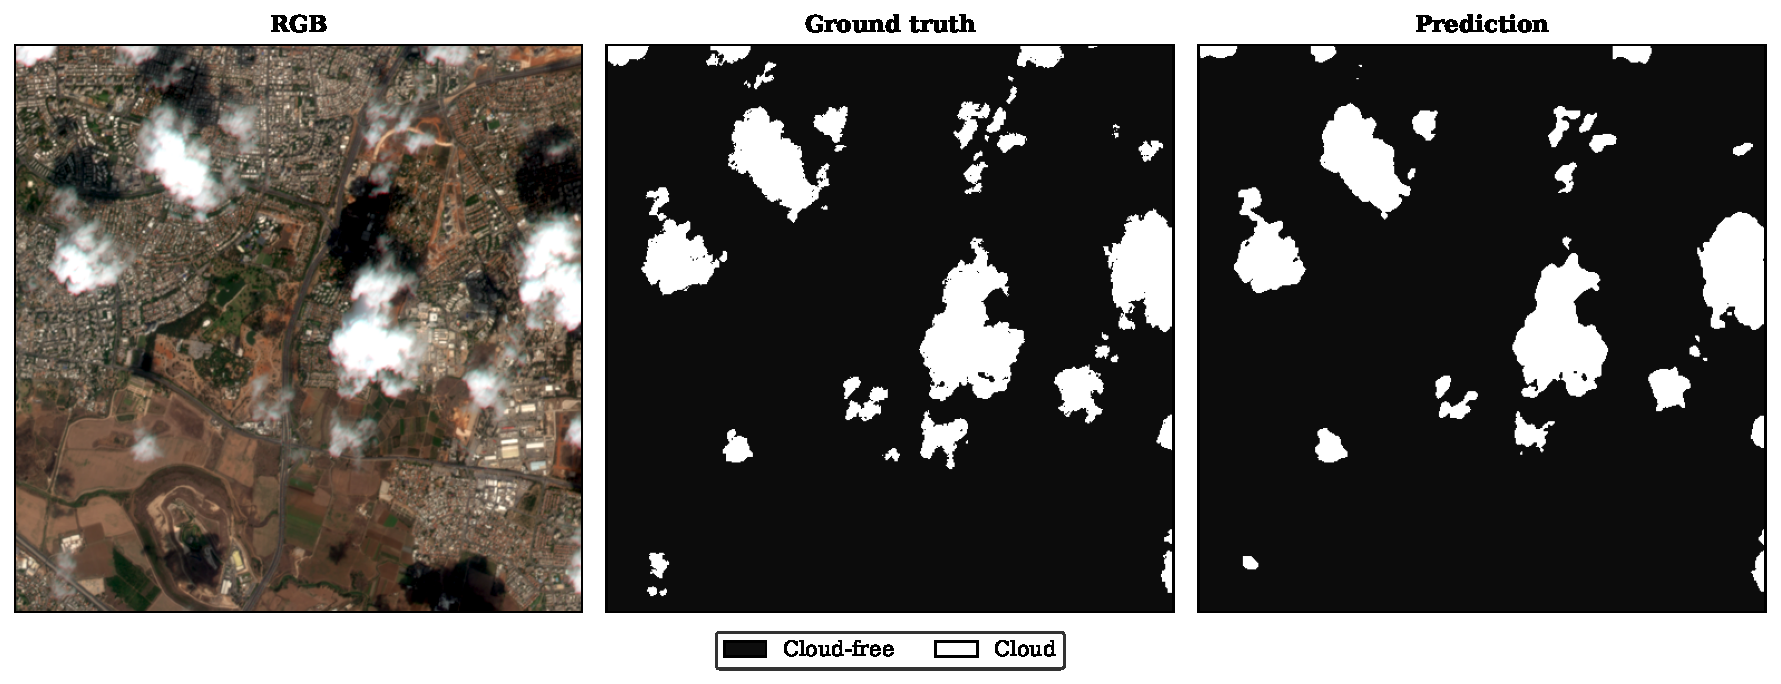
\includegraphics[width=0.98\textwidth]{text/img/e3_vis/w07_2048_0_0_1024_vis.pdf}
    \end{subfigure}
    \begin{subfigure}{\textwidth}
        \centering
        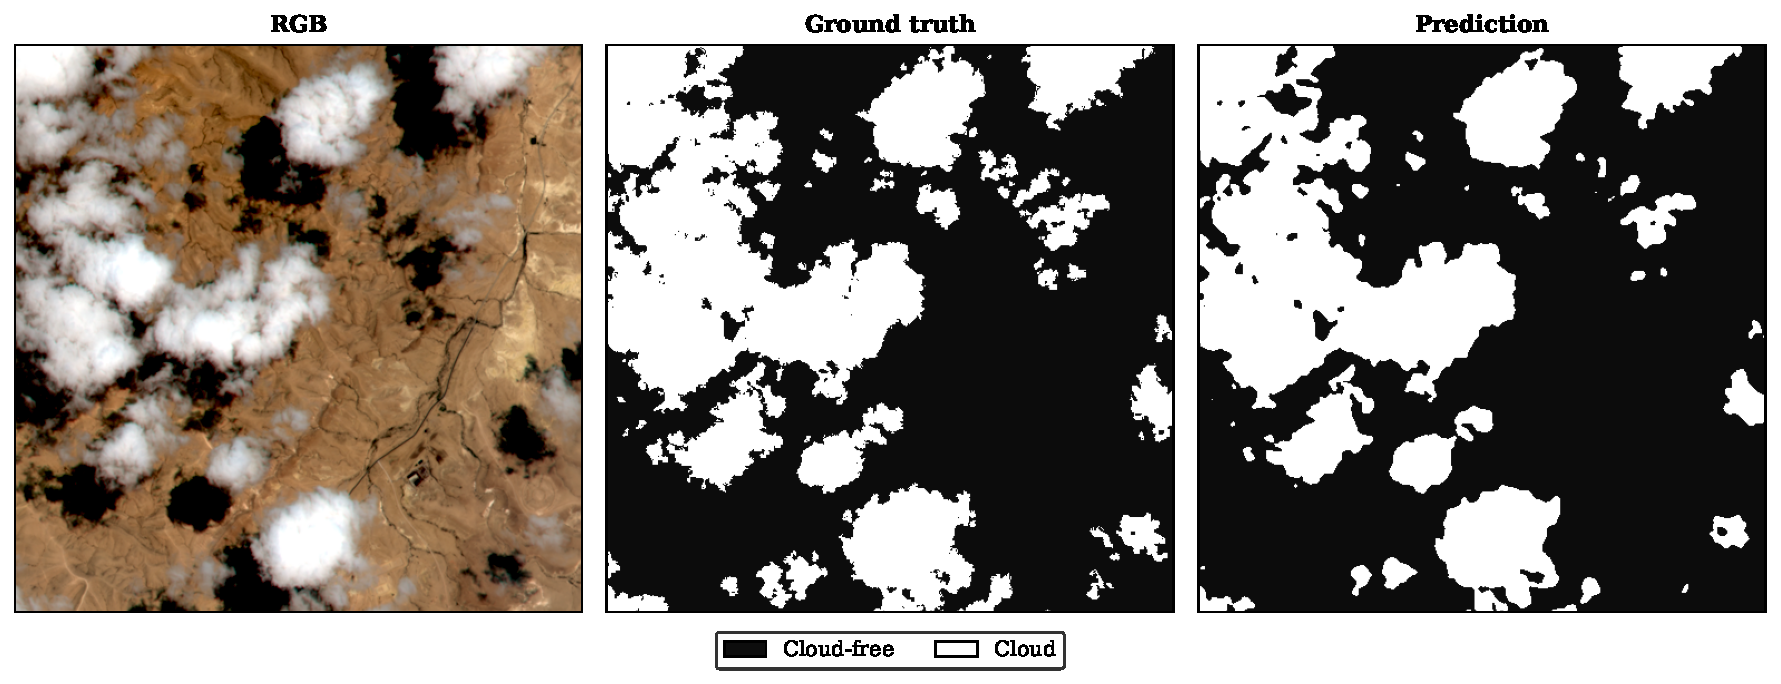
\includegraphics[width=0.98\textwidth]{text/img/e3_vis/s05_20180808_0_0_1024_0_vis.pdf}
    \end{subfigure}
    \begin{subfigure}{\textwidth}
        \centering
        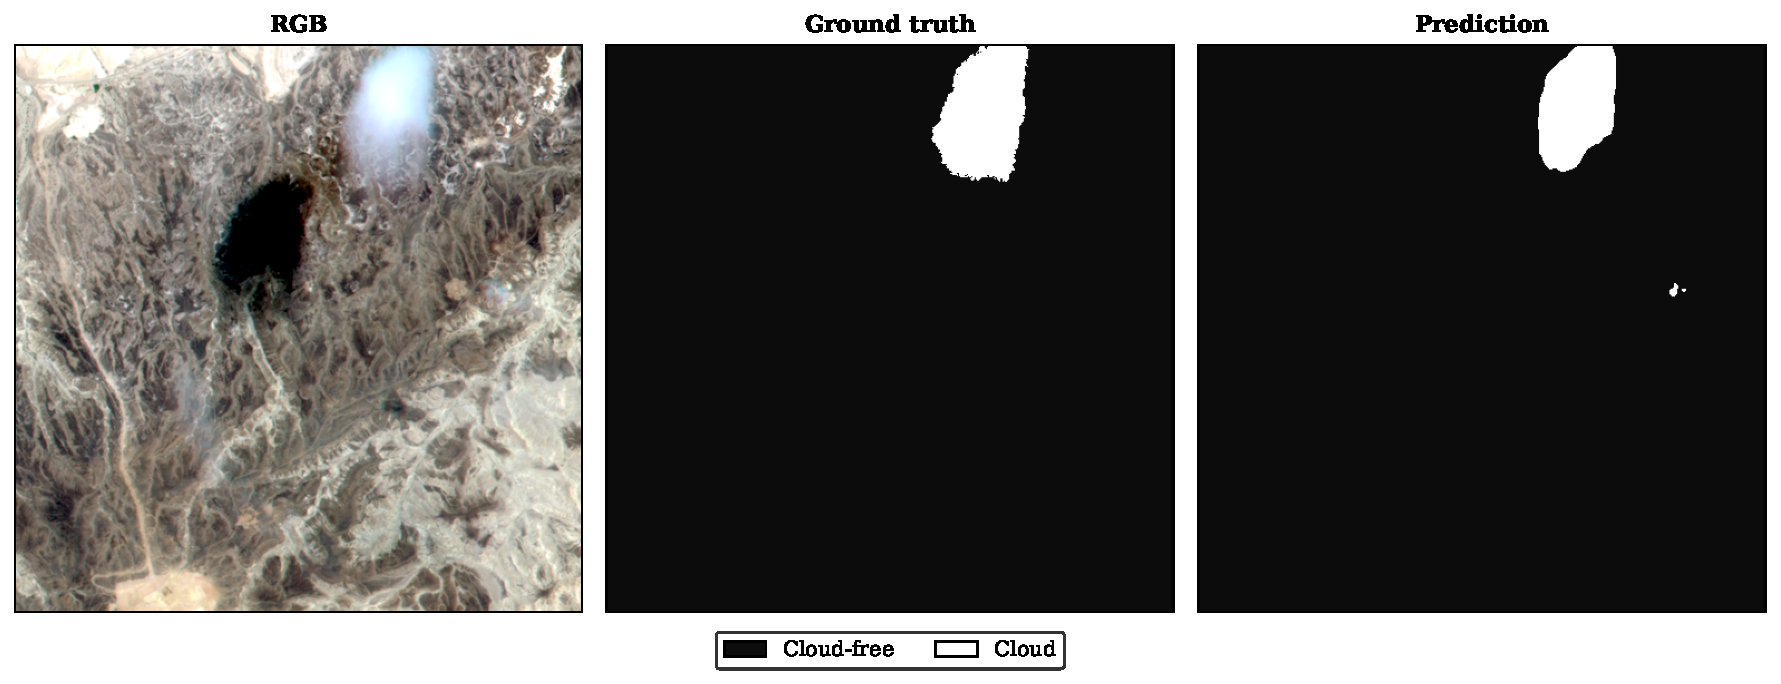
\includegraphics[width=0.98\textwidth]{text/img/e3_vis/s05_20180508_1793_1388_1024_512_vis.pdf}
    \end{subfigure}
    \caption[Additional prediction examples for full fine-tuning using dynamic Z-score normalization.]{Additional prediction examples for full fine-tuning using dynamic Z-score normalization on the VEN$\mu$S test set.}
    \label{fig:e3_visual_app}
\end{figure}

\addtocontents{toc}{\protect\setcounter{tocdepth}{1}}